\chapter{Introdução a Redes Neurais}
\label{ch:02-background}


% \epigraph{\itshape Those who cannot remember the past are condemned to compute it.''}{---Steven Pinker, \textit{Words and Rules}}

\section{Redes Neurais}

Uma rede neural é, essencialmente, um modelo de aprendizado de máquina supervisionado %[ref] 
que está a procura de aprender \textit{padrões}. Um modelo de aprendizado de máquina é uma tarefa computacional que explora algoritmos que podem aprender a partir de seus erros e fazer previsões sobre dados. A principal característica desse tipo de modelo é o caráter indutivo dos algoritmos, em oposição aos dedutivos. Esse tipo de algoritmo é normalmente inicializado com nenhuma expectativa sobre a tarefa que deve realizar e busca informações exclusivamente a partir dos dados do problema. Os possíveis tipos de aprendizado de máquina são divididos entre: \textit{supervisionados}, \textit{não-supervisionados} %ref
e por \textit{reforço}. %ref
No caso das redes neurais, o aprendizado diz-se supervisionado, pois informa-se à rede o \textit{output} esperado pelo treinamento.

A inspiração para o desenvolvimento desse tipo de modelagem surgiu a partir de estudos em neurosciência %[ref] 
que concluiram que, diante de múltiplas apresentações de um mesmo estímulo, um mesmo grupo de neurônios sofre incitação e dispara (\cite{hubel:1962}).  Analogamente, o modelo artificial é composto por uma camada de \textit{input} que recebe diferentes estímulos (representados em \ref{eq:sigmoid} por $\vect{x}$; vetores numéricos que representam o objeto a ser analisado). A informação recebida é distribuída ao longo de múltiplas conexões com a próxima camada através de uma múltiplicação com uma matriz de pesos $\vect{W}$. A matriz de pesos funciona como uma analogia às conexões existentes entre neurônios de modo que um peso maior representa uma conexão que deve ser reforçada e um peso menor representa uma conexão que deve ser reprimida. Além disso, é importante que o sistema de aprendizado não seja demasiado sensível a todo \textit{input} que receber, pois nesse caso cada \textit{input} diferente recebido alteraria completamente o modelo impossibilitando um aprendizado generalizado. Como solução, o resultado obtido a partir da multiplicação dos pesos pelos \textit{inputs} entra como argumento em uma função de ativação. A função de ativação é uma função que simula o potencial energético existente nas conexões neurais e permite que uma unidade apenas seja ativada caso o resultado dessa função atinja um \textit{threshold} mínimo. Isso permite ao sistema a produção de diferentes respostas para padrões diferentes utilizando a mesma rede e além disso, permite com que o aprendizado ocorra de forma gradual, de modo que o efeito de estímulos passados ainda perdure por um longo período mesmo após a apresentação de novos estímulos.
\begin{figure}[h]
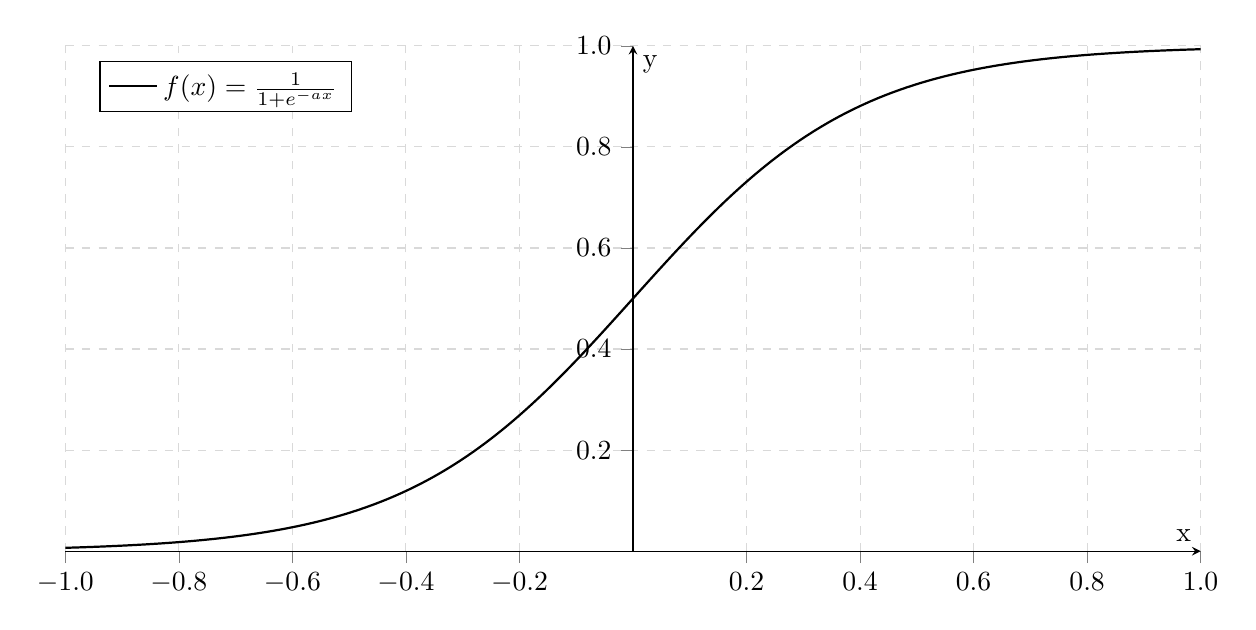
\begin{tikzpicture}
    \begin{axis}[
    	legend pos=north west,
        axis x line=middle,
        axis y line=middle,
        x tick label style={/pgf/number format/fixed,
                            /pgf/number format/fixed zerofill,
                            /pgf/number format/precision=1},
        y tick label style={/pgf/number format/fixed,
                            /pgf/number format/fixed zerofill,
                            /pgf/number format/precision=1},
        grid = major,
        width=16cm,
        height=8cm,
        grid style={dashed, gray!30},
        xmin=-1,     % start the diagram at this x-coordinate
        xmax= 1,    % end   the diagram at this x-coordinate
        ymin= 0,     % start the diagram at this y-coordinate
        ymax= 1,   % end   the diagram at this y-coordinate
        %axis background/.style={fill=white},
        xlabel=x,
        ylabel=y,
        tick align=outside,
        enlargelimits=false]
      % plot the stirling-formulae
      \addplot[domain=-1:1, black, thick,samples=500] {1/(1+exp(-5*x))};
      %\addplot[domain=-1:1, blue, ultra thick,samples=500] {1/(1+exp(-10*x))};
      \addlegendentry{$f(x)=\frac{1}{1+e^{-ax}}$}
      %\addlegendentry{$g(x)=\frac{1}{1+e^{-10x}}$}
    \end{axis} 
\end{tikzpicture}
\caption{A função logística utilizada para o cálculo da probabilidade de ativação.}
\label{fig:sigmoidplot}
\end{figure}

Uma das funções mais utilizadas na literatura é a função \textit{sigmoid}, uma função suave, diferenciável e facilmente interpretável (Fig. \ref{fig:sigmoidplot}). 

Após essa transformação, o resultado serve como novo input para a próxima camada e assim sucessivamente até a última, a camada de \textit{output}. Todas as camadas existentes entre as camadas de \textit{input} e de \textit{output} são chamadas de \textit{camadas escondidas} (Ver Fig. \ref{fig:ffd}.)

\begin{align}\label{eq:sigmoid}
p(w_{i} = 1) = \frac{1}{1+e^{\sum_{i} w_{i}x_{i}}}
\end{align}

Algebricamente, pode-se representar o processo descrito através da composição de múltiplas funções, uma vez que o resultado das operações precedentes servirão como entrada para as próximas camadas.

\begin{align}
f(\vect{x}) &= f^{(2)}(f^{(1)}(\vect{x}; \vect{W}_1); \vect{W}_2)\\
&= \sigma(\vect{W}_2 (\sigma(\vect{W}_1\vect{x})))
\end{align}

\definecolor{blue}{RGB}{159, 192, 176}
\definecolor{green}{RGB}{160, 227, 127}
\definecolor{orange}{RGB}{243, 188, 125}
\definecolor{red}{RGB}{253, 123, 84}
\definecolor{nephritis}{RGB}{39, 174, 96}
\definecolor{emerald}{RGB}{46, 204, 113}
\definecolor{turquoise}{RGB}{39, 174, 96}
\definecolor{green-sea}{RGB}{22, 160, 133}
\definecolor{purple}{RGB}{181, 124, 215}
% Tikzstyles for Computation Graphs

% nodes
\tikzstyle{noop} = [circle, draw=none, fill=red, minimum size = 10pt]
\tikzstyle{op} = [circle, draw=red, line width=1.5pt, fill=red!70, text=black, text centered, font=\bf \normalsize, minimum size = 25pt]

\tikzstyle{opintense} = [circle, draw=red, line width=1.5pt, fill=red!150, text=black, text centered, font=\bf \normalsize, minimum size = 25pt]


%new style
\tikzstyle{gp} = [circle, draw=red, line width=4pt, text=black, text centered, font=\bf \normalsize, minimum size = 4.cm]

\tikzstyle{box} = [rectangle, draw=red, line width=1.5pt, fill=red!70, text=black, align=center, font=\bf \normalsize, minimum size = 45pt]

\tikzstyle{state} = [circle, draw=blue, line width=1.5pt, fill=blue!70, text=black, text centered, font=\bf \normalsize, minimum size = 25pt]

\tikzstyle{output} = [circle, draw=purple, line width=1.5pt, fill=purple!70, text=black, text centered, font=\bf \normalsize, minimum size = 25pt]


\tikzstyle{gradient} = [circle, draw=nephritis, line width=1.5pt, fill=nephritis!60, text=black, text centered, font=\bf \normalsize, minimum size = 25pt]
\tikzstyle{textonly} = [draw=none, fill=none, text centered, font=\bf \normalsize]
\tikzstyle{boxtextonly} = [draw=none, fill=none, align=center, font=\bf \normalsize]

\tikzstyle{normal} = [circle, draw=black, line width=1.0pt, fill=none, text=black, text centered, font=\bf \normalsize, minimum size = 20pt]


% edges
\tikzstyle{tedge}  = [draw, thick, >=latex, ->]
\tikzstyle{tedge_dashed}  = [draw, thick, >=latex, ->, dashed]
\tikzstyle{nedge}  = [draw, thick, >=latex]
\tikzstyle{nedge_dashed}  = [draw, thick, >=latex, dashed]


% namedscope
\tikzstyle{namedscope} = [circle, draw=orange, line width=1.5pt, fill=orange!60, align=center, inner sep=0pt]
\begin{figure}[ht!]
\centering

\scalebox{1.0}{
\begin{tikzpicture}[auto]

% operations =========

% FNN input
\node[normal] (x1) {};
\node[textonly, above=10pt of x1] (input) {Camada de \textit{inputs}};
\node[normal, below=10pt of x1] (x2) {};
\node[normal, below=10pt of x2] (x3) {};
\node[normal, below=10pt of x3] (x4) {};
\node[normal, below=10pt of x4] (x5) {};
\node[normal, below=10pt of x5] (x6) {};

% FNN output
\node[textonly, right=50pt of x1] (center) {Camada Escondida};
\node[normal, below=25pt of center] (y1) {};
\node[normal, below=10pt of y1] (y2) {};
\node[normal, below=10pt of y2] (y3) {};

% FNN output
\node[textonly, right=110pt of input] (output) {Camada de \textit{outputs}};
\node[normal, below=15pt of output] (z1) {};

\node[normal, below=10pt of z1] (z2) {};
\node[normal, below=10pt of z2] (z3) {};
\node[normal, below=10pt of z3] (z4) {};
\node[normal, below=10pt of z4] (z5) {};
\node[normal, below=10pt of z5] (z6) {};

% phon features 2

% edges FNN
\path[nedge] (x1) -- (y1);
\path[nedge] (x1) -- (y2);
\path[nedge] (x1) -- (y3);

\path[nedge] (x2) -- (y1);
\path[nedge] (x2) -- (y2);
\path[nedge] (x2) -- (y3);

\path[nedge] (x3) -- (y1);
\path[nedge] (x3) -- (y2);
\path[nedge] (x3) -- (y3);

\path[nedge] (x4) -- (y1);
\path[nedge] (x4) -- (y2);
\path[nedge] (x4) -- (y3);

\path[nedge] (x5) -- (y1);
\path[nedge] (x5) -- (y2);
\path[nedge] (x5) -- (y3);

\path[nedge] (x6) -- (y1);
\path[nedge] (x6) -- (y2);
\path[nedge] (x6) -- (y3);

% edges FNN
\path[nedge] (y1) -- (z1);
\path[nedge] (y1) -- (z2);
\path[nedge] (y1) -- (z3);
\path[nedge] (y1) -- (z4);
\path[nedge] (y1) -- (z5);
\path[nedge] (y1) -- (z6);
\path[nedge] (y2) -- (z1);
\path[nedge] (y2) -- (z2);
\path[nedge] (y2) -- (z3);
\path[nedge] (y2) -- (z4);
\path[nedge] (y2) -- (z5);
\path[nedge] (y2) -- (z6);
\path[nedge] (y3) -- (z1);
\path[nedge] (y3) -- (z2);
\path[nedge] (y3) -- (z3);
\path[nedge] (y3) -- (z4);
\path[nedge] (y3) -- (z5);
\path[nedge] (y3) -- (z6);

\end{tikzpicture}
}\caption{Esquema de uma rede neural do tipo Feed-Forward} 
\label{fig:ffd}
\end{figure}

\subsection{Treinamento}

Para que a rede seja capaz de identificar os padrões desejados, é necessário alimentá-la com o que se espera como resposta (\textit{targets}), pois o treinamento da mesma consiste, essencialmente, na atualização das matrizes de pesos que deve ocorrer a partir da comparação entre os valores previstos pela rede (\textit{outputs}) e os \textit{targets}. A comparação entre esses valores se dá por meio de uma função de custo (\textit{Loss Function}), que representa uma forma de se quantificar o quão perto se está de uma rede ideal em que os resultados previstos correspondam exatamente aos \textit{targets}. O objetivo do aprendizado da rede é minimizar essa diferença, ou seja, encontrar o mínimo da função de custo (\cite{josh:2017}). Após a exposição a um certo número de exemplos, todos os pesos são atualizados simultaneamente com os valores que em conjunto minimizam a função de custo e portanto aproximam as previsões da rede aos \textit{targets}. %ref

\section{Modelo Apresentado em Rumelhart e McClelland (1986)}
\label{sec:arqFDD}

O esquema apresentado pelos pesquisadores Rumelhart e McClelland represetado na Fig. \ref{fig:esquemafdd} é conhecido como uma arquitetura do tipo \textit{Feed-Forward-Network (FFD)} sem camadas escondidas. Nesse caso, todos os nódulos da camada de input se conectam diretamente aos nódulos da camada de output.

Para uma melhor compreensão com relação à rede introduzida pelos autores, é necessário entender primeiramente o pré-processamento utilizado nos dados do treinamento, isto é, a análise dos verbos irregulares em unidades vetoriais simplificadas que alimentam o modelo computacional. Para tanto, é necessária a compreensão de um conceito introduzido pelos pesquisadores, o conceito de \textit{Wickelfeature}.

\subsection{Wickelfeatures}
\label{sec:wickelfeatures}
Os pesquisadores Rumelhart e McClelland propõem a caracterização de cada fonema como uma combinação simplificada de atributos em apenas 4 dimensões. O fonema \textit{d}, por exemplo, é caracterizado por um conjunto de 4 atributos: "Int.", indicando que é uma consoante interrompida; "V", indicando a vibração das cordas vocais; "Oclusi."  indicando que é uma consoante oclusiva; e "Média" por se tratar de um fonema produzido em ponto de articulação central. Seguindo este raciocínio para uma representação simplificada dos fonemas, os pesquisadores apresentam uma tabela que codifica cada fonema na língua inglesa às quatro dimensões de atributos. A Tabela \ref{tab:Tab1} foi baseada nesse sistema de codificação, porém com algumas adaptações para o português brasileiro. A tabela original apresentada pelos autores pode ser consultada no Apêndice. A primeira dimensão da tabela divide os fonemas em três grandes grupos: consoantes interrompidas, continuadas ou vogais. Dentre as consoantes interrompidas, encontram-se as consoantes oclusivas e nasais. Vê-se que nem todos os fonemas da tabela internacional (\ref{tab:ipa1} e \ref{tab:ipa2}) foram mapeados, apenas os mais importantes para a língua. Com relação às consoantes continuadas, estas foram subdivididas entre fricativas e líquidas (a versão dos autores ainda agrupava semi-vogais às líquidas). Ainda nesta dimensão, as vogais foram simplificadas a apenas altas ou baixas.  Com relação ao ponto de articulação (terceira dimensão), os autores agruparam bilabiais e labio-dentais em um único atributo entitulado de "anterior". Dentais e alveolares são consideradas consoantes com ponto de articulação médio. Pós-alveolares em diante são consideradas posteriores. A quarta dimensão subcategoriza as consoantes em vozeadas (V) vs. não-vozeadas (U) e as vogais em longas (L) e curtas (S). No caso da língua portuguesa não ocorre essa distinção entre as vogais, portanto essa dimensão é utilizada apenas para a dinstinção das vogais entre abertas e fechadas. No caso da vogal "u", ela representava a vogal curta associada à palavra \textit{book} (/buk/) e foi mantida nessa mesma posição.

A presença de cada um destes atributos em cada dimensão para um determinado fonema recebe o valor $1$, enquanto que a ausência, $0$. A primeira dimensão diz respeito à ordem Int - Cont - Vogal e um fonema é associado a um único atributo desta dimensão, ou seja, se o fonema for uma consoante interrompida, ele deve ser representado pelo vetor (100), se o fonema for uma consoante continuada, deve ser representado pelo vetor (010) e se for vogal, pelo vetor (001). O mesmo serve para as demais dimensões, sendo que a ordem da segunda é: Ocl - Nasal (dado que a primeira dimensão é uma consoante interrompida); Fricat - Liq (dado que a primeira dimensão é uma consoante continuada) ou Alta - Baixa caso a primeira dimensão aponte para uma vogal. Em seguida a terceira dimensão diz respeito à ordem: Anterior - Médio - Posterior. Por último, a interpretação da quarta dimensão também está condicionada à primeira dimensão, ou seja, caso o fonema seja uma consoante ele pode ser vozeado ou não-vozeado; caso seja uma vogal, longa ou curta. 
Com base na Tabela \ref{tab:Tab1}, portanto, o fonema \textit{d} passa a ser representado pelo vetor \ref{fond}. Cada sequência contida entre parênteses representa uma dimensão e os números dentro dela representam o atributo deste fonema nesta respectiva dimensão.

\begin{align}
d \Rightarrow (100)(10)(010)(10)\label{fond}
\end{align}

Com essa tabela o sistema de codificação para um único fonema está completo, porém é imprescindível que a própria sequência fonológica também seja representada já que cada fonema constitui parte de uma sequência e os padrões devem ser encontrados levando-se em consideração essa sequência. Desse modo, os pesquisadores optam por representar, em cada vetor de \textit{input}, uma sequência de três atributos (um trigrama de atributos) para cada uma das dimensões propostas (vogal - vogal - int, por exemplo). Além disso foi acrescentada uma última dimensão para representar início ou final de palavra, representado pelo símbolo "\#". Desse modo, \ref{token1}, \ref{token2} e \ref{token3} exibem as representações vetoriais do símbolo de fronteira e dos fonemas \textit{d} e \textit{a} considerando a última dimensão mencionada.

\begin{align}
\# \Rightarrow (000)(00)(000)(00)(1)\label{token1}\\
d \Rightarrow (100)(10)(010)(10)(0)\label{token2}\\
a \Rightarrow (001)(01)(010)(01)(0)\label{token3}
\end{align}

Por fim, define-se como um \textit{Wickelfeature} cada sequência de três atributos. Para alimentar a rede, os autores mapeiam cada verbo a um vetor booleano de tamanho 460, em que cada um destes valores representa a presença (ou ausência) de um \textit{Wickelfeature}. Em resumo, a rede completa é composta por duas camadas paralelas (\textit{input} e \textit{output} com 460 unidades de Wickelfeatures cada uma (Ver Fig. \ref{fig:esquemafdd}). 


\begin{table}[ht!]
\center
    \begin{tabular}{lrrrrrrr}\toprule
        &\multicolumn{2}{c}
{}&\multicolumn{1}{c}     {\textbf{Anterior}}&\multicolumn{2}{c}{\textbf{Médio}}&\multicolumn{2}{c}{\textbf{Posterior}}
        \\\cmidrule(r){3-4}\cmidrule(r){5-6}\cmidrule(r){7-8}   
        &&V/L&U/S&V/L&U/S&V/L&U/S\\\midrule
        Int.&   Oclusi. & b & p
                & d & t
                & g & k\\
                &Nasal & m
                & & n
                & & 
                & \\
        Cont. & Fricat. & v& f
                & z & s
                & j & S\\
                &Liq. &l
                & &r
                & &
                & h*\\
        Vogal & Alta & e & i 
                &   &  
                & o & u*\\
              & Baixa & a & E
              & &
              & & O
        \\\bottomrule
        Codificação: S = \ipa{S};&  j = \ipa{Z};& h\footnote{h* = Apesar de representar uma fricativa posterior, foi mantido nesta posição assim como na tabela proposta em \ref{fig:table-eng}} = x;& E = \textepsilon; & O = \textopeno & u\footnote{u* = u \& \textupsilon} & &
    \end{tabular}
    \caption{Categorização de fonemas em quatro dimensões adaptada ao Português Brasileiro}\label{tab:Tab1}
\end{table} 


\begin{center}
\scalebox{0.9}{
    \begin{tabular}{|l|cc|cc|cc|cc|cc|cc|cc|cc|cc|cc|cc|}
%\begin{tabular}{|l|cc|}
        \hline & 
            \multicolumn{2}{|c|}{\footnotesize{Bilabial}} &					% Bilabial
            \multicolumn{2}{|c|}{\footnotesize{Lab. dent.}} & 			% Labiodental
            \multicolumn{2}{|c|}{\footnotesize{Dental}} & 					% Dental
            \multicolumn{2}{|c|}{\footnotesize{Alveolar}} & 				% Alveolar
            \multicolumn{2}{|c|}{\footnotesize{P-alveo.}} & 		% Post-alveolar
            \multicolumn{2}{|c|}{\footnotesize{Retroflex}} & 				% Retroflex
            \multicolumn{2}{|c|}{\footnotesize{Palatal}} & 					% Palatal
            \multicolumn{2}{|c|}{\footnotesize{Velar}} & 					% Velar
            \multicolumn{2}{|c|}{\footnotesize{Uvular}} & 					% Uvular
            \multicolumn{2}{|c|}{\footnotesize{Pharyng.}} & 			% Pharyngeal
            \multicolumn{2}{|c|}{\footnotesize{Glottal}}  \\					% Glottal

        \hline Plosive &  							% Plosive
            p & b &													% Bilabial
            &&														% Labiodental
            \multicolumn{3}{|r}{t}&							% Dental
            \multicolumn{3}{l|}{d}&							% Alveolar
                                                                        % Post-alveolar
            \ipa{\:t} & \ipa{\:d}&									% Retroflex
            c & \textbardotlessj &														% Palatal
            k & g &													% Velar
            q & \ipa{\;G} &										% Uvular
            & \BlankCell        &								% Pharyngeal
            \ipa{P}& \BlankCell         \\								% Glottal

        \hline Nasal & 							% Nasal
            & m &													% Bilabial
            & \ipa{M} &											% Labiodental
            \multicolumn{3}{|r}{}&								% Dental
            \multicolumn{3}{l|}{n}&							% Alveolar
                                                                        % Post-alveolar
            & \ipa{\:n} &														% Retroflex
            & \textltailn &														% Palatal
            & \ipa{N} &														% Velar
            & \ipa{\;N} &														% Uvular
            \BlankCell        & \BlankCell        &		% Pharyngeal
            \BlankCell        & \BlankCell         \\		% Glottal

        \hline Trill &  								% Trill
            & \ipa{\;B}&											% Bilabial
            & &														% Labiodental
            \multicolumn{3}{|r}{}&								% Dental
            \multicolumn{3}{l|}{r}&								% Alveolar
                                                                        % Post-alveolar
            & &														% Retroflex
            & &														% Palatal
            \BlankCell        & \BlankCell        &		% Velar
            & \ipa{\;R}&											% Uvular
            & &														% Pharyngeal
            \BlankCell        & \BlankCell         \\		% Glottal

        \hline Tap/Flap &  						% Tap /Flap
            & &													% Bilabial
            & &														% Labiodental
            \multicolumn{3}{|r}{} &					% Dental
            \multicolumn{3}{l|}{\ipa{R}} &					% Alveolar
                                                                        % Post-alveolar
            & \ipa{\:r} &														% Retroflex
            & &														% Palatal
            \BlankCell        & \BlankCell        &		% Velar
            & &														% Uvular
            & &														% Pharyngeal
            \BlankCell        & \BlankCell         \\		% Glottal

        \hline Fricative & 						% Fricative
            \ipa{F} & \ipa{B} &									% Bilabial
            f & v &													% Labiodental
            \ipa{T} & \ipa{D} &									% Dental
            s & z &													% Alveolar
            \ipa{S} & \ipa{Z} &									% Post-alveolar
            \ipa{\:s} & \ipa{\:z} &								% Retroflex
            \ipa{\c{c}} & \ipa{J} &								% Palatal
            x & \ipa{G} &											% Velar
            \ipa{X} & \ipa{K} &									% Uvular
            \textcrh & \ipa{Q} &								% Pharyngeal
            h & \texthth \\										% Glottal

        \hline Lat. Fric. & 					% Lat. Fricative
            \BlankCell        & \BlankCell        &		% Bilabial
            \BlankCell        & \BlankCell        &		% Labiodental
            \multicolumn{3}{|r}{\textbeltl} &				% Dental
            \multicolumn{3}{l|}{\textlyoghlig} &			% Alveolar
                                                                        % Post-alveolar
            & &														% Retroflex
            & &														% Palatal
            & &														% Velar
            & &														% Uvular
            \BlankCell        & \BlankCell        			% Pharyngeal
            & \BlankCell        & \BlankCell         \\   % Glottal

        \hline Approx & 							% Approx.
            & &														% Bilabial
            & \ipa{V} &											% Labiodental
            \multicolumn{3}{|r}{}&								% Dental
            \multicolumn{3}{l|}{\ipa{\*r}} &					% Alveolar
                                                                        % Post-alveolar
            & \ipa{\:R} &											% Retroflex
            & j &														% Palatal
            & \textturnmrleg &									% Velar
            & &														% Uvular
            & &														% Pharyngeal
            \BlankCell        & \BlankCell         \\		% Glottal

        \hline Lat. appr. & 					% Lat. Approx
            \BlankCell        & \BlankCell        &		% Bilabial
            \BlankCell        & \BlankCell        &		% Labiodental
            \multicolumn{3}{|r}{}&								% Dental
            \multicolumn{3}{l|}{l}&								% Alveolar
                                                                        % Post-alveolar
            & \ipa{\:l} &											% Retroflex
            & \ipa{L} &												% Palatal
            & \ipa{\;L} &											% Velar
            & &														% Uvular
            \BlankCell        & \BlankCell        &		% Pharyngeal
            \BlankCell        & \BlankCell         \\		% Glottal
        \hline
    \end{tabular}
}%scalebox
\captionof{table}{Consoantes IPA}\label{tab:ipa1}
\end{center}

\begin{center}
    \begin{vowel}
        %    \putcvowel[l]{i}{1}
        \putvowel[l]{i}{0pt}{0pt}
        \putcvowel[r]{y}{1}
        \putcvowel[l]{e}{2}
        \putcvowel[r]{\o}{2}
        \putcvowel[l]{\textepsilon}{3}
        \putcvowel[r]{\oe}{3}
        \putcvowel[l]{a}{4}
        \putcvowel[r]{\textscoelig}{4}
        \putcvowel[l]{\textscripta}{5}
        \putcvowel[r]{\textturnscripta}{5}
        \putcvowel[l]{\textturnv}{6}
        \putcvowel[r]{\textopeno}{6}
        \putcvowel[l]{\textramshorns}{7}
        \putcvowel[r]{o}{7}
        \putcvowel[l]{\textturnm}{8}
        \putcvowel[r]{u}{8}
        \putcvowel[l]{\textbari}{9}
        \putcvowel[r]{\textbaru}{9}
        \putcvowel[l]{\textreve}{10}
        \putcvowel[r]{\textbaro}{10}
        \putcvowel{\textschwa}{11}
        \putcvowel[l]{\textrevepsilon}{12}
        \putcvowel[r]{\textcloserevepsilon}{12}
        \putcvowel{\textsci\ \textscy}{13}
        \putcvowel{\textupsilon}{14}
        \putcvowel{\textturna}{15}
        \putcvowel{\ae}{16}
    \end{vowel}
\captionof{table}{Vogais IPA}\label{tab:ipa2}   
\end{center} 


\subsection{Codificação}
\label{sec:cod}
Cada verbo que participa da etapa de treinamento da rede passa por um processo inicial de codificação. Tal processo é descrito a seguir utilizando o verbo \textit{dar} como exemplo.\\ 

\textbf{Entrada:} \textit{dar}\\

\textbf{Passo 1:} O token de início e final de palavra é acrescentado:\\
\hspace*{6.0em}      \#dar\#\\

\textbf{Passo 2:} O verbo é segmentado em trigramas:\\
\hspace*{6.0em}\#,d,a - d,a,r - a,r,\#\\

\textbf{Passo 3:} Um dicionário associa cada fonema a um vetor de features fonéticas, ou seja, toda possível combinação de features foi mapeada e associada a um índice de um dicionário. \\

\textbf{Passo 4:} As features dos trigramas são combinadas produzindo \textit{Wickelfeatures}.\\

%alterar a identacao aqui
Exemplos:
\begin{itemize}
\item \# - interrompida - vogal 
\item \# - oclusiva - baixa
\item \# - média - média
\item média - média - líquida
\item oclusiva - baixa - continuante
\item ...
\end{itemize}


\textbf{Passo 5:} Um dicionário de dimensão correspondente ao número total de \textit{Wickelfeatures} (460) é inicializado com $0's$ em todas as casas.\\

\textbf{Passo 6:} Cada \textit{Wickelfeature} presente no verbo analisado altera o valor do dicionário para $1$.\\

\textbf{Passo 7:} O dicionário resultante dos passos anteriores é utilizado como \textit{input} para a rede.

\subsection{Decodificação}
\label{sec:dec}

A primeira parte da decodificação da rede envolve a seleção das unidades de Wickelfeatures que compõe o início da palavra reconstituída. Primeiramente, selecionam-se todas as unidades que tem como primeiro atributo o indicador de fronteira '\#'. Em seguida, dentre estas, observam-se os Wickelfeatures com maior score. Feita esta seleção, os fonemas \textit{competem} pelas features, ou seja, todos os fonemas que compartilham de uma mesma feature observada somam pontos. Ao final deste processo, espera-se que o fonema com mais pontos seja o fonema alvo da decodificação. Decodificam-se portanto os primeiros dois fonemas.

A segunda parte do processo assemelha-se à primeira, porém ao invés da busca pelo trigrama inicial, selecionam-se todas as unidades que apresentam o atributo de fronteira na última posição. Em seguida ocorre o mesmo processo de competição para a decodificação dos dois últimos fonemas.

A terceira parte do processo de decodificação envolve uma busca de compatibilidade entre os atributos para os trigramas que não consitutem início ou final de palavra. Uma vez que o primeiro trigrama de fonemas foi decodificado, selecionam-se as próximas unidades cujas duas primeiras posições sejam compatíveis com as duas últimas do último trigrama decodificado. O processo de competição de fonemas se repete em um loop até que haja compatibilidade com o trigrama final, encontrado na segunda etapa.

O maior problema desta função de decodificação encontra-se na etapa da busca pelos trigramas que não constituem início ou fim de palavra. Dependendo da sequência, é possível que dois ou mais trigramas compartilhem de muitas unidades de Wickelfeatures, ou seja, se um Wickelfeature for ativado, não há como representar sua ativação uma segunda ou terceira vez, a sua ativação acontece apenas uma vez. Isto pode interferir na etapa de seleção de compatibilidades, fazendo com que a função não consiga sair do loop pois continua selecionando os mesmos Wickelfeatures. Esse problema já foi apontado por \cite{Pinker:1999}.
No livro, Pinker comenta a dificuldade da rede de Rumelhart e McClelland ao tentar decodificar a palavra 'algalgal' (uma palavra da língua Oykangand). Pinker faz uso desse exemplo pois, nesse caso, há inclusive a recorrência a nível de trigramas, mas o fato que é que mesmo a repetição a nível de \textit{Wickelfeatures} pode prejudicar a decodificação dos verbos. A probabilidade disso acontecer é ainda maior dependendo do comprimento dos verbos, e como apontado no Cap. \ref{ch:01-introduction}, os verbos da língua portuguesa possuem em média dois fonemas a mais que os verbos da língua inglesa. Como solução, foi necessária a implementação de uma função que considerasse apenas os trigramas fronteiriços. Desse modo foi possível verificar a capacidade da rede em capturar os processos de flexão irregulares que normalmente ocorrem no início ou no final das palavras. Para a palavra "postar", por exemplo, a irregularidade ocorre ao transmutar a vogal arredondada posterior semi-fechada para semi-aberta. Como essa irregularidade já pode ser detectada na primeira etapa da decodificação, pode-se avaliar o desempenho da rede baseado nesta etapa e desconsiderar a decodificação dos trigramas intermediários 'Ost' e 'stu' sem perda de informação.  

Para concluir, a implementação de uma rede FFD para a predição de irregularidades verbais do português brasileiro mostrou-se uma tarefa de grande dificuldade e motivou a construção de novos tipos de arquitetura para que se possa alcançar os objetivos propostos. 

\section{Encoder-Decoder}
\label{sec:enc-dec}

Uma vez que a arquitetura FFD gerou uma situação problemática, devido à própria natureza dos verbos em Português brasileiro somada às características do sistema de codificação dos fonemas e trigramas e seu posterior processamento, novas alternativas tiveram de ser investigadas. O problema, essencialmente, é relacionar sequências que influenciam umas às outras. Por exemplo, os verbos no infinitivo respeitam determinada lógica: são compostos por um radical mais um conjunto específico de terminações (\textit{ar, er, ir} e \textit{or}), e quando tal verbo é flexionado, é mandatório que determinadas regras relativas ao modo, tempo verbal e pessoa sejam respeitadas. Supondo que o verbo no infinitivo \textit{falar} seja conjugado na primeira pessoa do presente do indicativo, ou seja, \textit{falo}, neste caso, nota-se que o radical foi preservado e que a terminação foi alterada. Como esse processo de flexão verbal não é arbitrário e é possível inferir uma forma da outra, pode-se dizer que há um grau de subordinação entre os conjuntos de fonemas que compõe a forma infinitiva e a forma flexionada de cada verbo. Devido a uma condição fundamentalmente similar, uma analogia entre conjugação verbal e tradução de um idioma para outro pode ser estabelecida: ambos os processos obedecem a regras complexas consistentemente afim de preservar determinada coerência; na tradução a coerência semântica e sintática e na flexão verbal a lógica relativa a modo, tempo e pessoa. Visto que o problema é essencialmente o mesmo - processamento de sequências subordinadas - é de se supor que uma mesma técnica solucione ambas as situações, eis a implementação da função encoder-decoder, procedimento experimental utilizado, de acordo com a literatura mais atual (\cite{Goodfellow-et-al-2016}), em sistemas de tradução. Todavia, para a compreensão do funcionamento deste sistema, noções sobre Redes Neurais Recorrentes são indispensáveis, uma vez que a função encoder-decoder não passa de um mecanismo formado por tais redes.

\subsection{Redes Neurais Recorrentes}
\label{sec:RNN}

Na arquitetura FFD foi necessário acrescentar os indicadores de fronteira, e ainda, efetuar uma análise dos verbos em trigramas, ambos artifícios para tentar preservar a lógica sequencial. O insucesso desta estratégia motivou a implementação de um arquitetura melhor preparada para a realização da tarefa, as Redes Neurais Recorrentes (RNR).

A ideia central desse modelo consiste na retroalimentação dos elementos sequenciais, de modo que o \textit{input} de cada um deles serve, não somente para a previsão do próximo item da sequência, mas também para a formação de um componente intermediário, um \textit{estado}. Esses estados, representados na Figura \ref{fig:unfoldedrnn} como $\vect{h}$'s são matrizes que funcionam como uma espécie de memória condensada dos elementos precedentes e servem como input para os estados posteriores. Essa é uma maneira de retransmitir a cada momento os efeitos dos inputs anteriores para o restante da sequência (\cite{Goodfellow-et-al-2016}). 

%\definecolor{blue}{RGB}{159, 192, 176}
\definecolor{green}{RGB}{160, 227, 127}
\definecolor{orange}{RGB}{243, 188, 125}
\definecolor{red}{RGB}{253, 123, 84}
\definecolor{nephritis}{RGB}{39, 174, 96}
\definecolor{emerald}{RGB}{46, 204, 113}
\definecolor{turquoise}{RGB}{39, 174, 96}
\definecolor{green-sea}{RGB}{22, 160, 133}
\definecolor{purple}{RGB}{181, 124, 215}
% Tikzstyles for Computation Graphs

% nodes
\tikzstyle{noop} = [circle, draw=none, fill=red, minimum size = 10pt]
\tikzstyle{op} = [circle, draw=red, line width=1.5pt, fill=red!70, text=black, text centered, font=\bf \normalsize, minimum size = 25pt]

\tikzstyle{opintense} = [circle, draw=red, line width=1.5pt, fill=red!150, text=black, text centered, font=\bf \normalsize, minimum size = 25pt]


%new style
\tikzstyle{gp} = [circle, draw=red, line width=4pt, text=black, text centered, font=\bf \normalsize, minimum size = 4.cm]

\tikzstyle{box} = [rectangle, draw=red, line width=1.5pt, fill=red!70, text=black, align=center, font=\bf \normalsize, minimum size = 45pt]

\tikzstyle{state} = [circle, draw=blue, line width=1.5pt, fill=blue!70, text=black, text centered, font=\bf \normalsize, minimum size = 25pt]

\tikzstyle{output} = [circle, draw=purple, line width=1.5pt, fill=purple!70, text=black, text centered, font=\bf \normalsize, minimum size = 25pt]


\tikzstyle{gradient} = [circle, draw=nephritis, line width=1.5pt, fill=nephritis!60, text=black, text centered, font=\bf \normalsize, minimum size = 25pt]
\tikzstyle{textonly} = [draw=none, fill=none, text centered, font=\bf \normalsize]
\tikzstyle{boxtextonly} = [draw=none, fill=none, align=center, font=\bf \normalsize]

\tikzstyle{normal} = [circle, draw=black, line width=1.0pt, fill=none, text=black, text centered, font=\bf \normalsize, minimum size = 20pt]


% edges
\tikzstyle{tedge}  = [draw, thick, >=latex, ->]
\tikzstyle{tedge_dashed}  = [draw, thick, >=latex, ->, dashed]
\tikzstyle{nedge}  = [draw, thick, >=latex]
\tikzstyle{nedge_dashed}  = [draw, thick, >=latex, dashed]


% namedscope
\tikzstyle{namedscope} = [circle, draw=orange, line width=1.5pt, fill=orange!60, align=center, inner sep=0pt]
\begin{figure}[ht!]
\centering

\scalebox{1.40}{
\begin{tikzpicture}[auto]

% RNN state cell =============================
\node[normal] (h) {$\vect{h}$};
\node[normal, below=30pt of h] (x) {$\vect{x}$};
\node[normal, above=30pt of h] (yhat) {$\hat{\vect{y}}$};



% edges
\path[tedge] (x) edge node[below right= -4pt] {}  (h) ;
\path[tedge] (h) edge [out=-400,in=-320,looseness=8, distance=125pt] node[above right] {} (h);
\path[tedge] (h) edge node[below right = -4pt] {} (yhat);


\end{tikzpicture}

} % scalebox
\caption{Representação Simplificada de uma RNN}
\label{fig:RNN1}
\end{figure}
\definecolor{blue}{RGB}{159, 192, 176}
\definecolor{green}{RGB}{160, 227, 127}
\definecolor{orange}{RGB}{243, 188, 125}
\definecolor{red}{RGB}{253, 123, 84}
\definecolor{nephritis}{RGB}{39, 174, 96}
\definecolor{emerald}{RGB}{46, 204, 113}
\definecolor{turquoise}{RGB}{39, 174, 96}
\definecolor{green-sea}{RGB}{22, 160, 133}
\definecolor{purple}{RGB}{181, 124, 215}
% Tikzstyles for Computation Graphs

% nodes
\tikzstyle{noop} = [circle, draw=none, fill=red, minimum size = 10pt]
\tikzstyle{op} = [circle, draw=red, line width=1.5pt, fill=red!70, text=black, text centered, font=\bf \normalsize, minimum size = 25pt]

\tikzstyle{opintense} = [circle, draw=red, line width=1.5pt, fill=red!150, text=black, text centered, font=\bf \normalsize, minimum size = 25pt]


%new style
\tikzstyle{gp} = [circle, draw=red, line width=4pt, text=black, text centered, font=\bf \normalsize, minimum size = 4.cm]

\tikzstyle{box} = [rectangle, draw=red, line width=1.5pt, fill=red!70, text=black, align=center, font=\bf \normalsize, minimum size = 45pt]

\tikzstyle{state} = [circle, draw=blue, line width=1.5pt, fill=blue!70, text=black, text centered, font=\bf \normalsize, minimum size = 25pt]

\tikzstyle{output} = [circle, draw=purple, line width=1.5pt, fill=purple!70, text=black, text centered, font=\bf \normalsize, minimum size = 25pt]


\tikzstyle{gradient} = [circle, draw=nephritis, line width=1.5pt, fill=nephritis!60, text=black, text centered, font=\bf \normalsize, minimum size = 25pt]
\tikzstyle{textonly} = [draw=none, fill=none, text centered, font=\bf \normalsize]
\tikzstyle{boxtextonly} = [draw=none, fill=none, align=center, font=\bf \normalsize]

\tikzstyle{normal} = [circle, draw=black, line width=1.0pt, fill=none, text=black, text centered, font=\bf \normalsize, minimum size = 20pt]


% edges
\tikzstyle{tedge}  = [draw, thick, >=latex, ->]
\tikzstyle{tedge_dashed}  = [draw, thick, >=latex, ->, dashed]
\tikzstyle{nedge}  = [draw, thick, >=latex]
\tikzstyle{nedge_dashed}  = [draw, thick, >=latex, dashed]


% namedscope
\tikzstyle{namedscope} = [circle, draw=orange, line width=1.5pt, fill=orange!60, align=center, inner sep=0pt]

% RNN STATE CELL ====================================

\newcommand{\rnnSimple}[4]{

% operations
\node[normal, minimum size=40pt,#4] (h#3) {$\vect{h}^{#1}$};
\node[normal, minimum size=40pt,below=30pt of h#3] (x#3) {$\vect{x}^{#1}$};
\node[normal, minimum size=40pt, above=30pt of h#3] (yhat#3) {$\hat{\vect{y}}^{#1}$};

% edges
\path[tedge] (x#3) edge node[below right= -4pt] {} (h#3);
\path[tedge] (h#3) edge node[below right = -4pt] {} (yhat#3);
}

\begin{figure}[ht!]
\centering
\hspace*{-1.0cm}
\scalebox{0.9}{
\begin{tikzpicture}[auto]

% timestep 1
\rnnSimple{(1)}{(0)}{t1}{}

% % timestep 0
\node[normal, minimum size=40pt,left=50pt of ht1] (ht0) {$\vect{h}^{(0)}$};

% % timestep 2
\rnnSimple{(2)}{(1)}{t2}{right=50pt of ht1};


% % timestep 2
\rnnSimple{(3)}{(1)}{t3}{right=50pt of ht2};


% % state transfers
\path[tedge] (ht0) edge node[above right = 2pt] {} (ht1);
\path[tedge] (ht1) edge node[above right = 2pt] {} (ht2);
\path[tedge] (ht2) edge node[above right = 2pt] {} (ht3);

\end{tikzpicture}
}%\scalebox
\caption{Representação Expandida de uma RNN}
\label{fig:unfoldedrnn}
\end{figure}




Os estados indicados na Fig. \ref{fig:unfoldedrnn} são calculados a partir da equação recorrente\footnote{O estado $\vect{h(0)}$ é normalmente inicializado de maneira aleatória.}:

\begin{equation}
\vect{h}^{(t)} = g(\vect{h}^{(t-1)}, \vect{x}^{(t)}; \vect{\theta})
\label{eq:rnn}
\end{equation}

Na prática, essa arquitetura simplificaria algumas das etapas do processo de predição de irregularidades verbais. A primeira delas seria o processo de codificação dos verbos, por exemplo, ao se utilizar uma rede recorrente, indicadores de fronteira e a ativação de unidades em trigramas não se fazem mais necessários. No treinamento desse tipo de rede, os inputs são gerados a partir de cada item da série, e os alvos, por sua vez, são os itens subsequentes respectivos. Isto significa, essencialmente, que a rede será treinada para prever item a item de uma sequência. O alvo mais simples para este tipo de processamento são fonemas, uma vez que traços fonológicos ou Wickelfeatures, por serem intrinsecamente mais complexos, exigiriam uma arquitetura de rede muito mais sofisticada. Por fim, o processo de decodificação dos verbos também torna-se desnecessário uma vez que o output é computado item após item. A Fig. \ref{fig:rnnpractice} ilustra o problema da predição de fonemas dada uma base de verbos flexionados. No exemplo, considera-se o treinamento do verbo \textit{"pa.r\textupsilon"}. 

% Apesar da praticidade desse tipo de rede, ela infelizmente apresenta alguns problemas para tarefas que envolvem dependências de longa distância, o que normalmente é o caso quando se trata de tarefas linguísticas. O problema ocorre porque, a cada \textit{input}, as matrizes de pesos são atualizadas fazendo com que as últimas informações recebidas sejam mais relevantes do que as anteriores, impedindo o progresso do treinamento. Dessa forma, apresentam-se na literatura algumas soluções. Entre elas, uma arquitetura conhecida como \textit{Long Short-Term Memory - LSTM}.

\definecolor{blue}{RGB}{159, 192, 176}
\definecolor{green}{RGB}{160, 227, 127}
\definecolor{orange}{RGB}{243, 188, 125}
\definecolor{red}{RGB}{253, 123, 84}
\definecolor{nephritis}{RGB}{39, 174, 96}
\definecolor{emerald}{RGB}{46, 204, 113}
\definecolor{turquoise}{RGB}{39, 174, 96}
\definecolor{green-sea}{RGB}{22, 160, 133}
\definecolor{purple}{RGB}{181, 124, 215}
% Tikzstyles for Computation Graphs

% nodes
\tikzstyle{noop} = [circle, draw=none, fill=red, minimum size = 10pt]
\tikzstyle{op} = [circle, draw=red, line width=1.5pt, fill=red!70, text=black, text centered, font=\bf \normalsize, minimum size = 25pt]

\tikzstyle{opintense} = [circle, draw=red, line width=1.5pt, fill=red!150, text=black, text centered, font=\bf \normalsize, minimum size = 25pt]


%new style
\tikzstyle{gp} = [circle, draw=red, line width=4pt, text=black, text centered, font=\bf \normalsize, minimum size = 4.cm]

\tikzstyle{box} = [rectangle, draw=red, line width=1.5pt, fill=red!70, text=black, align=center, font=\bf \normalsize, minimum size = 45pt]

\tikzstyle{state} = [circle, draw=blue, line width=1.5pt, fill=blue!70, text=black, text centered, font=\bf \normalsize, minimum size = 25pt]

\tikzstyle{output} = [circle, draw=purple, line width=1.5pt, fill=purple!70, text=black, text centered, font=\bf \normalsize, minimum size = 25pt]


\tikzstyle{gradient} = [circle, draw=nephritis, line width=1.5pt, fill=nephritis!60, text=black, text centered, font=\bf \normalsize, minimum size = 25pt]
\tikzstyle{textonly} = [draw=none, fill=none, text centered, font=\bf \normalsize]
\tikzstyle{boxtextonly} = [draw=none, fill=none, align=center, font=\bf \normalsize]

\tikzstyle{normal} = [circle, draw=black, line width=1.0pt, fill=none, text=black, text centered, font=\bf \normalsize, minimum size = 20pt]


% edges
\tikzstyle{tedge}  = [draw, thick, >=latex, ->]
\tikzstyle{tedge_dashed}  = [draw, thick, >=latex, ->, dashed]
\tikzstyle{nedge}  = [draw, thick, >=latex]
\tikzstyle{nedge_dashed}  = [draw, thick, >=latex, dashed]


% namedscope
\tikzstyle{namedscope} = [circle, draw=orange, line width=1.5pt, fill=orange!60, align=center, inner sep=0pt]

% RNN STATE CELL ====================================

\begin{figure}[ht!]
\centering
\hspace*{-1.0cm}
\scalebox{0.9}{
\begin{tikzpicture}[auto]

% timestep 1
\rnnSimple{(1)}{(0)}{t1}{}

% % timestep 0
\node[normal, minimum size=40pt,left=50pt of ht1] (ht0) {$\vect{h}^{(0)}$};

% % timestep 2
\rnnSimple{(2)}{(1)}{t2}{right=50pt of ht1};
\node[textonly, below= 80pt of ht1] (p) {p};
\node[textonly, above= 80pt of ht1] (â) {a};

% % timestep 2
\rnnSimple{(3)}{(1)}{t3}{right=50pt of ht2};
\node[textonly, below= 80pt of ht2] (a) {a};
\node[textonly, above= 80pt of ht2] (r_o) {r};

% % state transfers
\path[tedge] (ht0) edge node[above right = 2pt] {} (ht1);
\path[tedge] (ht1) edge node[above right = 2pt] {} (ht2);
\path[tedge] (ht2) edge node[above right = 2pt] {} (ht3);

% timestep3
\node[textonly, below= 80pt of ht3] (r) {r};
\node[textonly, above= 80pt of ht3] (end) {\textupsilon};

\end{tikzpicture}
}%\scalebox
\caption{RNN - Modelo de Linguagem}
\label{fig:rnnpractice}
\end{figure}




% \subsection{Long Short-Term Memory}
% \label{sec:LSTM}

% Uma LSTM continua sendo uma RNN, porém existem algumas especificidades em sua arquitetura que a tornam mais elaborada e mais adequada para atender aos treinamentos que envolvem longa dependência. A chave para entender como as LSTM's lidam com esse problema está no entendimento de um componente chamado de \textit{cell state}. Esse componente funciona como uma corrente transportadora de informação e é regulado por estruturas que funcionam como válvulas (os \textit{gates}). Os \textit{gates} são uma forma de filtragem de informação. Eles são basicamente responsáveis por selecionar informações antigas que podem ser esquecidas e novas que sejam relevantes. 

% %imagem de LSTM
% \begin{figure}[ht!]
\centering
\begin{tikzpicture}[
    % GLOBAL CFG
    font=\sf \scriptsize,
    >=LaTeX,
    % Styles
    cell/.style={% For the main box
        rectangle, 
        rounded corners=5mm, 
        draw,
        very thick,
        },
    operator/.style={%For operators like +  and  x
        circle,
        draw,
        inner sep=-0.5pt,
        minimum height =.2cm,
        },
    function/.style={%For functions
        ellipse,
        draw,
        inner sep=1pt
        },
    ct/.style={% For external inputs and outputs
        circle,
        draw,
        line width = .75pt,
        minimum width=1cm,
        inner sep=1pt,
        },
    gt/.style={% For internal inputs
        rectangle,
        draw,
        minimum width=4mm,
        minimum height=3mm,
        inner sep=1pt
        },
    mylabel/.style={% something new that I have learned
        font=\scriptsize\sffamily
        },
    ArrowC1/.style={% Arrows with rounded corners
        rounded corners=.25cm,
        thick,
        },
    ArrowC2/.style={% Arrows with big rounded corners
        rounded corners=.5cm,
        thick,
        },
    ]

%Start drawing the thing...    
    % Draw the cell: 
    \node [cell, minimum height =4cm, minimum width=6cm] at (0,0){} ;

    % Draw inputs named ibox#
    \node [gt] (ibox1) at (-2,-0.75) {$\sigma$};
    \node [gt] (ibox2) at (-1.5,-0.75) {$\sigma$};
    \node [gt, minimum width=1cm] (ibox3) at (-0.5,-0.75) {Tanh};
    \node [gt] (ibox4) at (0.5,-0.75) {$\sigma$};

   % Draw opérators   named mux# , add# and func#
    \node [operator] (mux1) at (-2,1.5) {$\times$};
    \node [operator] (add1) at (-0.5,1.5) {+};
    \node [operator] (mux2) at (-0.5,0) {$\times$};
    \node [operator] (mux3) at (1.5,0) {$\times$};
    \node [function] (func1) at (1.5,0.75) {Tanh};

    % Draw External inputs? named as basis c,h,x
    \node[ct, label={[mylabel]Cell State (t-1)}] (c) at (-4,1.5) {\empt{c}{t-1}};
    \node[ct, label={[mylabel]Estado de (t-1)}] (h) at (-4,-1.5) {\empt{h}{t-1}};
    \node[ct, label={[mylabel]left:Input}] (x) at (-2.5,-3) {\empt{x}{t}};

    % Draw External outputs? named as basis c2,h2,x2
    \node[ct, label={[mylabel] Cell State (t)}] (c2) at (4,1.5) {\empt{c}{t}};
    \node[ct, label={[mylabel] Estado (t) }] (h2) at (4,-1.5) {\empt{h}{t}};
    \node[ct, label={[mylabel]left: Estado (t)}] (x2) at (2.5,3) {\empt{h}{t}};

% Start connecting all.
    %Intersections and displacements are used. 
    % Drawing arrows    
    \draw [ArrowC1] (c) -- (mux1) -- (add1) -- (c2);

    % Inputs
    \draw [ArrowC2] (h) -| (ibox4);
    \draw [ArrowC1] (h -| ibox1)++(-0.5,0) -| (ibox1); 
    \draw [ArrowC1] (h -| ibox2)++(-0.5,0) -| (ibox2);
    \draw [ArrowC1] (h -| ibox3)++(-0.5,0) -| (ibox3);
    \draw [ArrowC1] (x) -- (x |- h)-| (ibox3);

    % Internal
    \draw [->, ArrowC2] (ibox1) -- (mux1);
    \draw [->, ArrowC2] (ibox2) |- (mux2);
    \draw [->, ArrowC2] (ibox3) -- (mux2);
    \draw [->, ArrowC2] (ibox4) |- (mux3);
    \draw [->, ArrowC2] (mux2) -- (add1);
    \draw [->, ArrowC1] (add1 -| func1)++(-0.5,0) -| (func1);
    \draw [->, ArrowC2] (func1) -- (mux3);

    %Outputs
    \draw [-, ArrowC2] (mux3) |- (h2);
    \draw (c2 -| x2) ++(0,-0.1) coordinate (i1);
    \draw [-, ArrowC2] (h2 -| x2)++(-0.5,0) -| (i1);
    \draw [-, ArrowC2] (i1)++(0,0.2) -- (x2);

\end{tikzpicture}
\caption{Rede Neural LSTM} \label{fig:lstm}
\end{figure}

% A Fig. \ref{fig:lstm} deve ser interpretada da seguinte forma: A cada novo input ($x(t)$), uma camada LSTM recebe o estado $h(t-1)$ gerado pelo input anterior assim como uma RNN comum receberia, mas recebe também o Cell State de (t-1). O Cell State traz consigo uma lista de todas as informações que ele considera que devem ser carregadas e mantidas durante todo o treinamento. Após a intervenção dos gates, o modelo pode decidir por agregar novas informações e esquecer outras nessa lista, gerando assim um novo Cell State (t). Além disso, a passagem desse input por essa camada também gera um novo estado ($h(t)$) que, além de servir como referência para o cálculo do output de (t), servirá também como referência para o próximo processamento ($x(t+1)$). (\cite{Goodfellow-et-al-2016})

% \section{Encoder-Decoder}
% \label{sec:enc-dec}
\section{perai}
Um modelo de mapeamento Encoder-Decoder é um sistema composto por duas RNNs cuja principal função é mapear sequências. A primeira rede, chamada encoder, mapeia os dados de uma determinada sequência de origem e os transforma em uma representação codificada, esta alimenta então a segunda rede, decoder, que, por sua vez, tem como objetivo gerar uma nova sequência alvo.  %ref
Modelos do tipo Encoder-Decoder (também conhecidos como \textit{Seq2Seq}) tem sido bastante utilizados em tarefas linguísticas, especialmente no desenvolvimento de sistemas de diálogo e em tradução automática. Em um contexto de tradução do inglês para o português, por exemplo, uma rede encoder seria treinada com um corpus em inglês, o qual apresenta determinadas probabilidades de arranjo sintático e valores semânticos, ou seja, uma gestalt sequencial armazenada em uma matriz. A rede decoder, ao ser treinada na língua alvo, isto é, português, implicitamente leva em consideração tanto as características sintático-semânticas desta quanto a gestalt da rede encoder, gerando desta forma uma nova sequência que contempla ambas as línguas e assemelha-se a uma tradução humana. Tecnicamente, a gestalt gerada pela rede encoder nada mais é do que o último estado consolidado alcançado a partir dos treinamentos dessa rede. A decoder, portanto, recebe como input, não só os exemplos da língua alvo como também o estado gerado pela rede encoder. Por fim, obtem-se um sistema capaz de predizer os resultados de uma sequência alvo a partir de uma sequência de origem.

Em função de uma similaridade conceitual, este modelo foi escolhido, uma vez que possibilita uma interação mediada pela essência de duas qualidades de padrões sequencias e tem como objetivo a produção de um resultado orgânico, semelhante, por exemplo, a intuição de um falante nativo que advinha a conjugação da primeira pessoa do presente a partir de um verbo no infinitivo. 
\begin{figure}[ht!]
\centering

\scalebox{1.0}{
\begin{tikzpicture}[
  hid/.style 2 args={
    rectangle split,
    rectangle split horizontal,
    draw=#2,
    rectangle split parts=#1,
    fill=#2!20,
    outer sep=1mm}]
  % draw input nodes
  \foreach \i [count=\step from 1] in {the,cute,kitten,{{$<$eos$>$}}}
    \node (i\step) at (2*\step, -2) {\i};
  % draw output nodes
  \foreach \t [count=\step from 4] in {o,gatinho,fofo,{{$<$eos$>$}}} {
    \node[align=center] (o\step) at (2*\step, +2.75) {\t};
  }
  % draw embedding and hidden layers for text input
  \foreach \step in {1,...,3} {
    \node[hid={3}{red}] (h\step) at (2*\step, 0) {};
    \node[hid={3}{red}] (e\step) at (2*\step, -1) {};    
    \draw[->] (i\step.north) -> (e\step.south);
    \draw[->] (e\step.north) -> (h\step.south);
  }
  % draw embedding and hidden layers for label input
  \foreach \step in {4,...,7} {
    \node[hid={3}{yellow}] (s\step) at (2*\step, 1.25) {};
    \node[hid={3}{blue}] (h\step) at (2*\step, 0) {};
    \node[hid={3}{blue}] (e\step) at (2*\step, -1) {};    
    \draw[->] (e\step.north) -> (h\step.south);
    \draw[->] (h\step.north) -> (s\step.south);
    \draw[->] (s\step.north) -> (o\step.south);
  }  
  % edge case: draw edge for special input token
  \draw[->] (i4.north) -> (e4.south);
  % draw recurrent links
  \foreach \step in {1,...,6} {
    \pgfmathtruncatemacro{\next}{add(\step,1)}
    \draw[->] (h\step.east) -> (h\next.west);
  }
  % draw predicted-labels-as-inputs links
  \foreach \step in {4,...,6} {
    \pgfmathtruncatemacro{\next}{add(\step,1)}
    \path (o\step.north) edge[->,out=45,in=225] (e\next.south);
  }
\end{tikzpicture}
}\caption{Esquema de Encoder-Decoder para Tradução Automática} 
\label{fig:seq2seq}
\end{figure}




